\section{Theoretische Grundlagen}

\subsection{Polarisationszustände des Lichts}

Aus den Maxwellgleichungen ergeben sich als allgemeine Lösungen die ebenen Wellen, gegeben durch
$$\vec E = \vec{E_0}\cdot \cos(\omega t - kz)$$
wobei o.B.d.A k in z-Richtung liegt. Der Vektor $\vec{E_0} \perp \vec k$ beschreibt somit wie das E-Feld orientiert ist. Bei einer Lichtwelle gilt genau das gleiche noch einmal für das B-Feld, darauf gehen wir aber jetzt nicht näher ein, da es komplett analog ist.

Für $\vec{E}$ gibt es 3 mögliche Polarisationszustände:

\begin{itemize}

\item Lineare Polarisation: Das E-Feld zeigt immer in die gleiche Richtung, d.h. die $x$- und die $y$-Komponenten schwingen in Phase:
$ \vec{E} = \begin{pmatrix} E_{0x} \\ E_{0y} \\ 0 \end{pmatrix}\cdot\cos(\omega t-kz) $

\item Zirkulare Polarisation: Das E-Feld dreht sich um seine Propagationsachse, d.h. dass die Beträge der $x$- un $y$-Komponenten gleich sind, ihre Phase jedoch um 90$^\circ$ verschoben ist:
$\vec{E}= E_0\cdot \begin{pmatrix} \cos(\omega t - kz) \\ \sin(\omega t - kz) \\ 0 \end{pmatrix}$

\item Elliptische Polarisation: In allen anderen Fällen ist das Licht elliptisch polarisiert.
\end{itemize}

Bei linear polarisiertem Licht, lässt sich die Ebene des E-Felds am einfachsten mit einem Polarisator nachweisen. Die Intensität des Lichts hinter einem Polarisationsfilter (Analysator) sagt aus wie der Winkel des E-Felds zu dem Filter orientiert ist. Die maximale Intensität erhält man, wenn diese beiden Winkel sich genau entsprechen. Die Intensität kann man z.B. mit einer Photodiode messen.
Eine andere Möglichkeit ist der Halbschattenpolarimeter. Desen Vorteil liegt darin, dass man mit dem menschlichen Auge die Polarisation überprüfen kann. Ein Teil des polarisierten Lichts wird um einen Winkel zu dem anderen Teil gedreht. Hinter dem Analysator sieht der Betrachter zwei unterschiedliche Flächen. Der Analysator wird gedreht, bis die Flächen nicht mehr unterscheidbar sind, und man kann dann den Winkel der Polarisation, bzw. dessen Änderung, ablesen.




\subsection{Doppelbrechung}

\begin{figure}[H]
	\centering 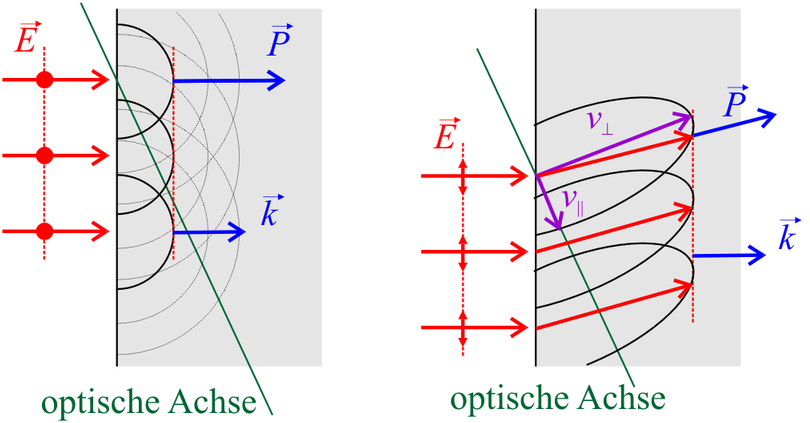
\includegraphics[width = 0.8\textwidth]{Bilder/Doppelbrechung.jpg}
	\caption{Doppelbrechung \emph{(wikipedia.de)}}
\end{figure}

In einem anisotropen Medium sind Ausbreitungsrichtung der Welle und Energieflussrichtung verschieden. Der Brechungsindex ist abhängig von der Raumrichtung und somit werden verschieden polarisierte Wellen anders gebrochen. Einfallendes Licht wird in zwei Teilbündel gespalten, wovon ein Teil dem Snelliusschen Brechungsindex beim Eintreten in das Medium gehorcht (ordentlicher Strahl), der andere Teil nicht (außerordentlicher Strahl). Beide Strahlen sind senkrecht zueinander polarisiert. Die ordentliche Welle ist senkrecht und die außerordentliche Welle ist parallel zu optischen Achse des Kristalls polarisiert.


\subsection{Piezoeffekt}

In bestimmten Materialien, piezoelektrisch genannt, entstehen durch Verformung mikroskopische Dipole in diesen, die eine Spannung induzieren. Da sehr viele dieser Dipole entstehen, ist die Spannung sogar messbar. Dieser Effekt tritt allerdings auch in umgekehrter Form auf, legt man an piezoelektrische Materialien eine Spannung an, so verformen sich diese. Über den Photoelastischen Effekt wirkt sich dies auch auf den Brechungsindex aus. Durch Symmetrieüberlegungen lässt sich zeigen, dass dieser Effekt nur für Kristalle ohne Symmetriezentrum existiert.


\subsection{Pockelseffekt}

Die dielektrische Konstante ist definiert durch 

\begin{equation} \epsilon = \frac{\partial D}{\partial E}  \end{equation}
\begin{equation} \text{mit \ } D = aE + bE^2 + cE^3 + \dots \end{equation}

$\epsilon$ ist also eigentlich keine Konstante und $D$ hängt nicht linear von $E$ ab. Für $\epsilon$ folgt also:
\begin{equation} \epsilon = a + 2bE + 3cE^2 + \dots \end{equation}

Der Term $3cE^2$ ist verantwortlich für den Kerr-Effekt und ebenso wie alle Terme höherer Ordnung in unserem Versuch vernachlässigbar klein. Der Parameter $b$ fasst hier zwei verschiedene Effekte zusammen. Er beschreibt einerseits den Pockelseffekt, die \emph{direkte lineare Veränderung der dielektrischen Verschiebung} durch das externe Feld. Andererseits zeigt aber auch der Piezoeffekt eine lineare Abhängigkeit von der Feldstärke und wird somit ebenso durch diesen Parameter beschrieben. Somit stört uns dieser bei der Messung des reinen Pockelseffekts. Da er auf Veränderungen der Gitterstruktur beruht, welche wesentlich langsamer sind als die direkte Änderung der dielektrischen Verschiebung, versuchen wir ihn durch hinreichend hochfrequente Signale zu elimienieren.

Der Pockels-Effekt existiert ebenso wie der Piezo-Effekt nur für Kristalle ohne Symmetriezentrum.



\subsection{Faradayeffekt}

Legt man ein durchsichtiges isotropes Medium in ein longitudinales Magnetfeld, so wird das Medium optisch aktiv. Rechtszirkulare Lichtwellen und linkszirkulare Lichtwellen propagieren mit verschiedenen Geschwindigkeiten. Schickt man also eine linear polarisierte Wellen durch das Medium (linear polarisierte Wellen bestehen aus gegenseitig zirkular polarisierten Wellen), so kommt diese wegen der Phasenverschiebung der beiden Teilwellen in einem Winkel $\alpha$ zu dem Winkel, mit dem es eingefallen ist, heraus. Der Winkel $\alpha$ ist gegeben durch:

\begin{equation} \alpha = V\cdot l \cdot H \end{equation}

$H$ ist hier die magnetische Feldstärke des longitudinalen Feldes und $l$ die Länge des Mediums. $V$ wird als Verdet-Konstante bezeichnet und hängt von der Wellenlänge und der Dispersion ab.

\subsection{Magnetfeld einer Spule}

Fließt ein Strom durch einen Draht, erzeugt dieser ein Magnetfeld, welches in einer Ebene senkrecht zum Stromfluss gegen den Uhrzeigersinn im Kreis fließt. Das Magnetfeld lässt sich mit dem Ampèreschen Gesetz berechnen:

\begin{equation} \oint \vec B \cdot ds = \mu_0\cdot I \end{equation}

Für das Feld außerhalb eines geraden Drahtes ergibt sich somit (näherungsweise):

$$B(r) = \frac{\mu_0\cdot I}{2\pi\cdot r} $$

Für eine Spule, hängt das Feld von der Anzahl der Windungen N ab. Nähert man die Spule als lang genug (Länge $L$), so ergibt sich aus dem Ampèreschen Gesetz für das Innere der Spule:

\begin{equation} B = \frac{\mu_0\cdot N\cdot I}{L} \end{equation}


\begin{figure}[H]
	\centering 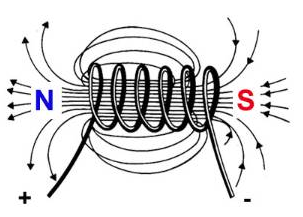
\includegraphics[width = 0.5\textwidth]{Bilder/Spule.jpg}
	\caption{Das Magnetfeld einer Spule \emph{(paukr.de)}}
\end{figure}

Wie man sehen kann, ist das B-Feld im Innern einer Spule also homogen und unabhängig vom Ort.

Ist die Spule allerdings nicht hinreichend lang im Verhältnis zum betrachteten Gebiet, erhält man eine Abhängigkeit von der Position entlang der Spulenachse, sowie einigen weiteren geometrischen Eigenschaften der Spule. Über das Biot-Savart-Gesetz
$$  dH\left( z \right) = \frac{1}{4 \pi} \frac{I d\vec{l} \times \vec{r}}{\left|r\right|^3} $$
erhält man
$$ H \left( z \right) = \frac{N I}{2 L \left( x_2 - x_1 \right)} \left( \left( L - z \right) \ln \frac{x_2 + \sqrt{\left( L-z \right)^2 + x_2^2}}{x_1 + \sqrt{\left( L - z \right)^2 + x_1^2}} + z \ln \frac{x_2 + \sqrt{z^2 + x_2^2}}{x_1 + \sqrt{z^2 + x_1^2}}  \right) $$

Für uns interresant ist das Integral über die Stablänge
$$ \int_{\frac{L-l}{2}}^{\frac{L+l}{2}} H\left( z \right) dz = 2556 I $$
wobei der genaue Zahlenwert natürlich nur für die spezifischen Eigenschaften unseres Aufbaus gilt. Die Herleitung findet sich in der Staatsexamensarbeit.


\clearpage